\documentclass[tikz, border = 2pt]{standalone}

%---------------------------------------------------------------------------%
% PACKAGES                                                                  %
%---------------------------------------------------------------------------%

%----- MATH
%---------------------------------------------------------------------------%
\usepackage{amsmath, amssymb}
%----- FIGURES
%---------------------------------------------------------------------------%
\usepackage{pgfplots}
\pgfplotsset{compat=1.13}


\begin{document}

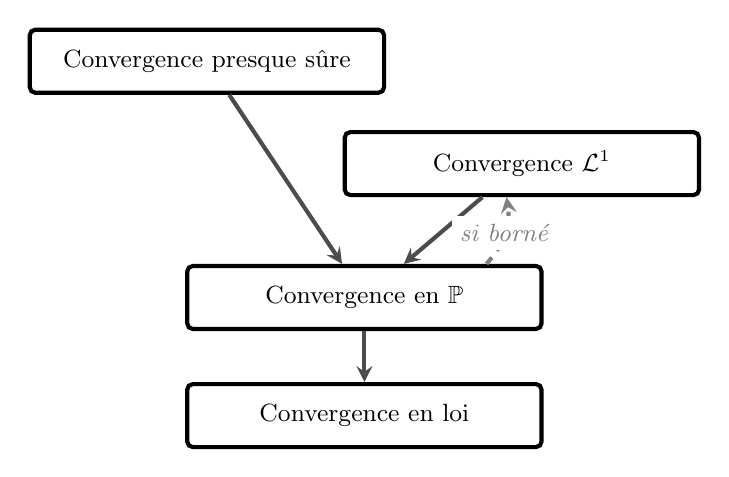
\begin{tikzpicture}
% définition des styles
\tikzstyle{quadri}=[rectangle, draw=black, fill=white, line width=1.5pt, rounded corners=2pt, minimum width=4.5cm, minimum height=0.8cm, font=\small]
\tikzstyle{implique}=[->, >=stealth, thick, line width=1.5pt, color=black!70]
\tikzstyle{impliquecond}=[->, >=stealth, line width=1.5pt, color=black!50, dashed]

% les nœuds
\node[quadri] (PS) at (0,0) {Convergence presque sûre};
\node[quadri] (M) at (4,-1.3) {Convergence $\mathcal{L}^1$};
\node[quadri] (P) at (2,-3) {Convergence en $\mathbb{P}$};
\node[quadri] (L) at (2,-4.5) {Convergence en loi};

% les flèches
\draw[implique] (PS)--(P);
\draw[implique] (M)--(P); 
\draw[implique] (P)--(L);
\draw[impliquecond] (P) to[bend right=25] node[midway, fill=white, inner sep=3pt, font=\small]{\textit{si borné}} (M);

% la légende
\end{tikzpicture}

\end{document}